\section{Bodenabfertigungen eines Luftfahrzeugs}
\label{s:Bodenabfertigungen eines Luftfahrzeugs}

Zur Veranschaulichung der Änderungen an der Infrastruktur am Flughafen die durch neuartige Antriebe vorgenommen werden müssen, 
ist es notwendig wichtige Begriffe einer Abfertigung des konventionellen Flugzeugs hervorzuheben (definieren). 
Unter konventionellen Luftfahrzeugen sind die zu verstehen,
die mit fossilen Treibstoffen, wie Kerosin, betrieben werden. Der Fokus wird auf die gewerblichen Passagier-Flugzeuge gelegt,
weil die Abfertigung von Passagieren besonders strengere Sicherheitsmaßnahmen erfordert.

%Nach der Reinigung der Kabine (Boeing B747-400 im Transit bis zu 45 min), Toiletten und Frischwasser nachfüllen und Catering
%Boarding ca. 15-20 min pro 100 PAX

Die Blockzeit setzt sich aus der Zeit vom Beginn der Bewegung von der Parkposition bis zum Ende der Bewegung zur Parkposition, 
einschließlich der Flugzeit, zusammen.

An der Parkposition des Flughafens werden die Triebwerke ausgeschaltet und der Ablauf eines Turnaround beginnt. 
Mensen \cite{mensen2013handbuch} definiert den Turnaround, wie die Abfertigung der Flüge, die zeitnah zusammen liegen.
Bei einem Turnaround wird das Luftfahrzeug durch viele Akteure am Flughafen, wie Flugplatzbetreiber, Fluggesellschaft und die Dritte, für 
den nächsten Flug vorbereitet \cite{mensen2013handbuch}. Es muss ausgeladen, kontrolliert, gereinigt, anschließend versorgt 
und für den nächsten Flug beladen werden. \\
\\
Die Abbildung \ref{abfertigung} stellt die Abfertigung eines Flugzeugs an der Parkposition dar.
Nach ICAO Doc 9157: besteht Abfertigung eines Passagierflugzeugs aus Passagier-, Gepäck- und Frachtabfertigung, 
Sanitärservice, Wasserbetankung, Gepäckabfertigung, Betankung, Stromversorgung,
Startluft?, Schleppen von Flugzeugen, Bordküchenservice, Wartungsservice sowie Bereitstellung einer Klimaanlage und Sauerstoff,
wie in der Abbildung dargestellt.

Das Flugzeug wird an ein Hilfstriebwerk (auxiliary power unit - APU) angeschlossen \cite{mensen2013handbuch}. 
Die APU liefert Strom, wenn die Haupttriebwerke nicht laufen (quelle: [Annex 14. Doc 9137 Part 8]).
Parallel werden Fracht und sonstige Gepäckeinheiten mit dem Hubwagen abgeladen und mit Transporthängern zur Sortieranlage 
im Terminal gebracht \cite{mensen2013handbuch}. Im Falle, das die Parkposition direkt am Flughafen ist, 
können Passagiere direkt über die Treppe oder Fluggastbrücke zum Terminalgebäude gelangen. 
Wenn die Parkposition am Vorfeld liegt, muss auf einen Bus zurückgegriffen werden. 
Laut EU-OPS 1.305 darf das Luftfahrzeug aus Sicherheitsgründen erst betankt werden, wenn die Passagiere sich nicht an Bord befinden. 
%ICAO empfiehlt in Annex 6, dass Flugzeuge sollen erst betankt werden, wenn alle Passagiere raus sind 
%Das Flugzeug wird abgefertigt und wenn die Flüge zeitnan zusammen liegen beginnt ein Turn Around (TA) \cite{mensen2013handbuch}, 

\begin{figure}[h]
	\centering
	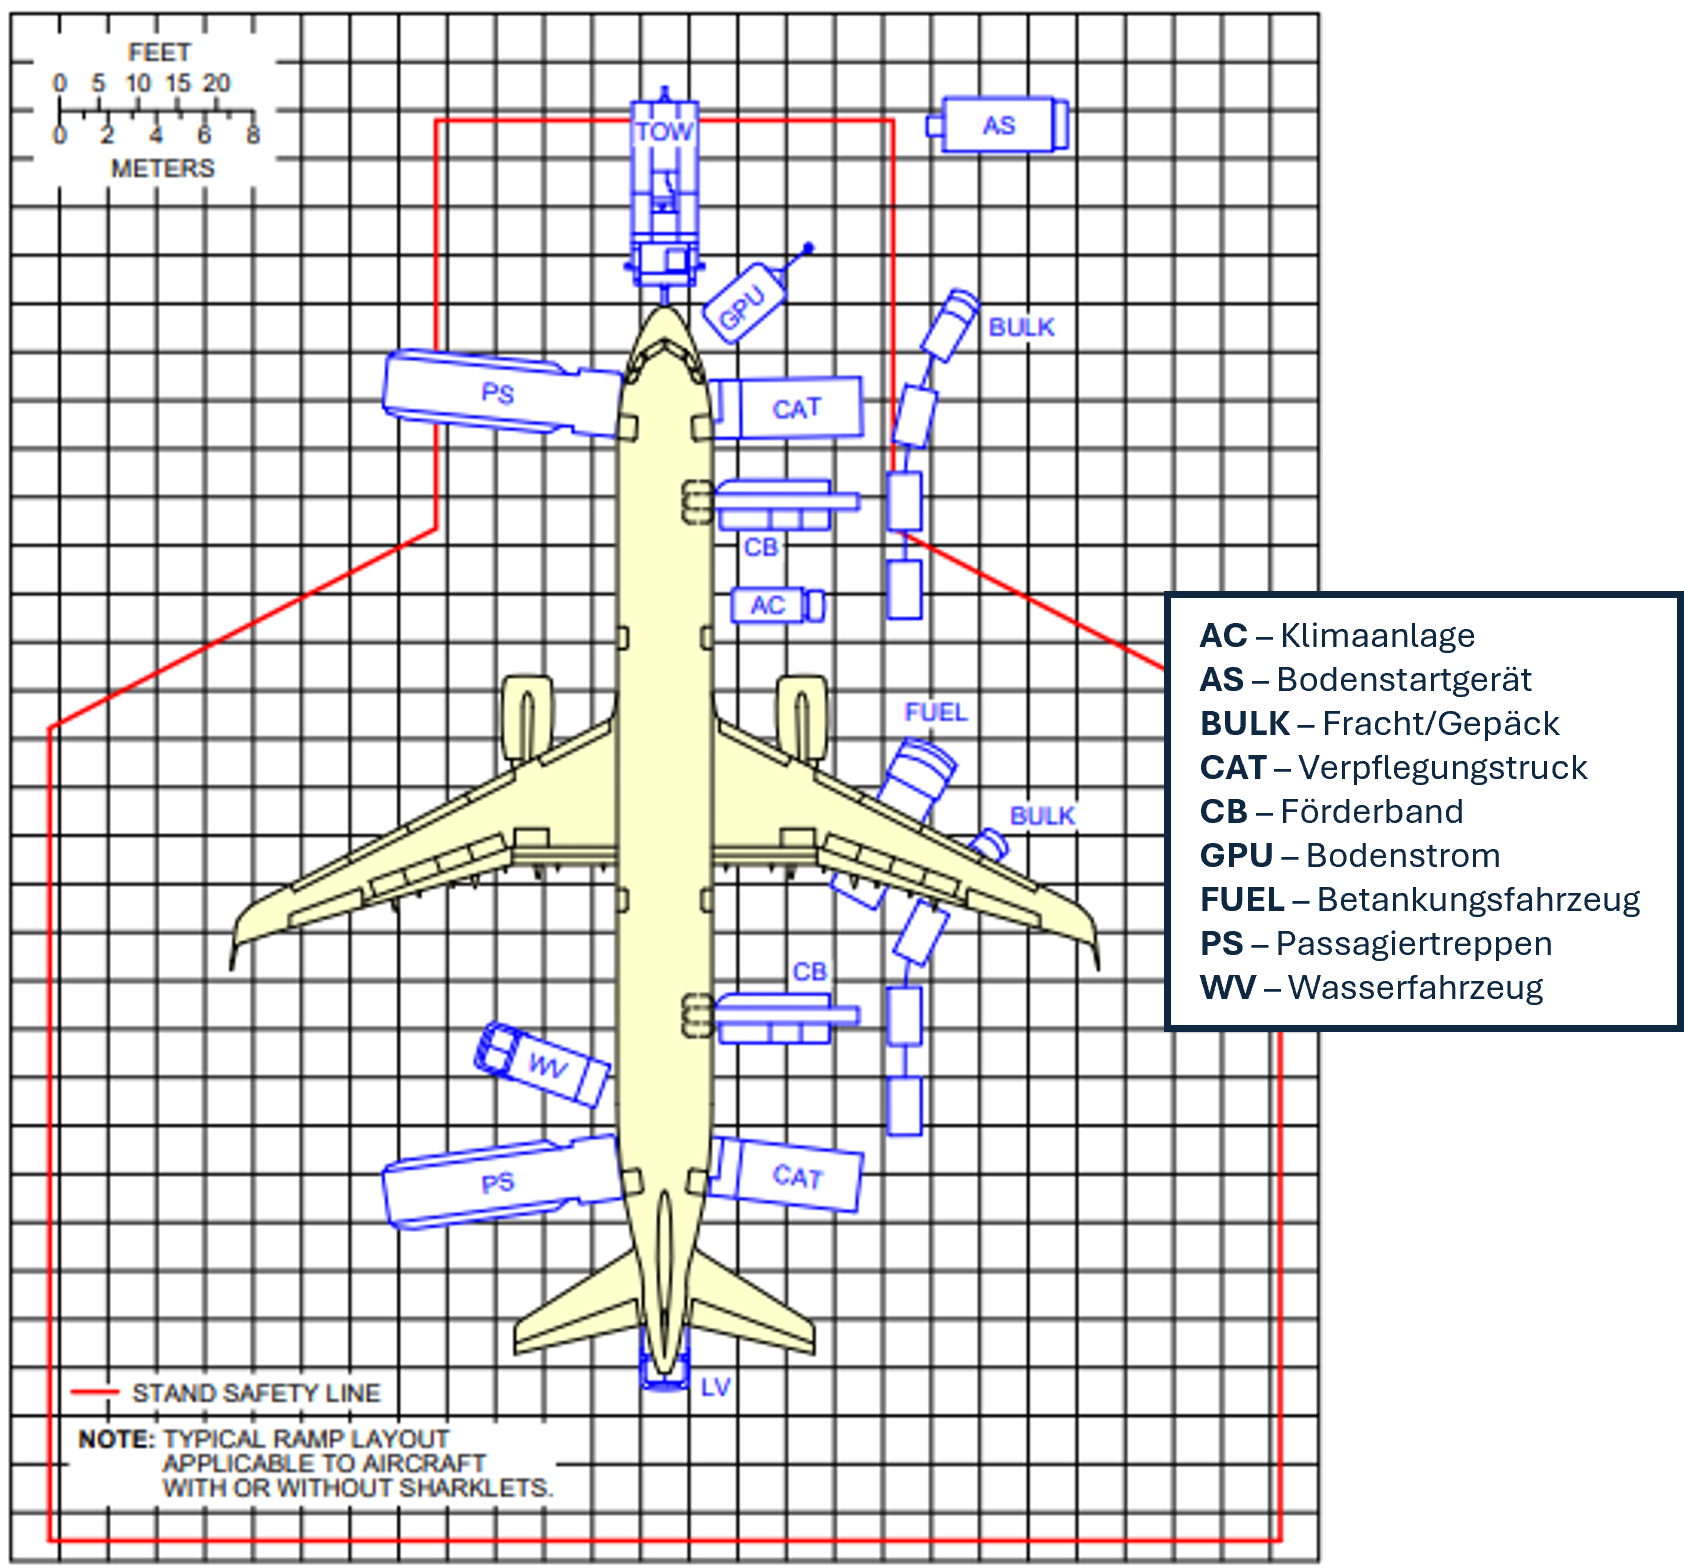
\includegraphics[width=0.8\linewidth]{Bilder/A321_Abfertigung.png}
	\caption[Abfertigung]{Abfertigung eines A321 \cite{airbus2022a321} mit eigenem Hinweis}
	\label{abfertigung}
\end{figure}

%"Die TurnaroundTime ist die Zeit vom Andocken des Flugzeugs amGate bis zumAbrollenvomGate." \cite{conrady2019luftverkehr} S 368

%Fluggast- Fracht-, und Postabfertigung 
%Fluggastabfertigung beinhaltet alles um den Service für die Passagiere.

Je nach Flugdistanz und nach Flugzeuggröße kann es zu unterschiedlichen Abfertigungszeiten kommen. Bei einem kleineren Flugzeug ist die Dauer 
kürzer als bei einer größeren Maschine. 
In Bezug auf die Transportdistanz unterscheidet man nach Kurz- (ca.2 Stunden oder bis 1000 km) 
und Mittelstreckenflüge (bis 3,5 Stunden oder bis 3000 km), Langstreckenflüge (ab 3,5 Stunden und ab 3000 km) \cite{mensen2013handbuch}.
Der Flughafen Frankfurt definiert jedoch die Transportdistanz anders, diese Werte werden auch im Kapitel \ref{s:Betriebsszenarien} genutzt.


